\subsection{Red Doméstica}

Para la primera captura, se eligió la red domestica de uno de los integrantes del grupo. Los dispositivos conectados a la red en este caso fueron, 3 computadoras, 2 teléfonos celulares, un televisor SmartTV y un Apple TV. Todos estos conectados al modem del proveedor de internet.
La captura duró aproximadamente 30 minutos.
En Figura~\ref{fig:red_domestica_network}. se pueden observar los diferentes nodos de la red asociados a su dirección IP. Los ejes que conectan a un par de nodos representan que ellos hubo algún envío de paquetes. El tamaño de cada nodo es proporcional a la cantidad de paquetes el mismo envió y recibió.
\\
Al ser una red pequeña podemos distinguir claramente a los nodos distinguidos. El que posee la dirección IP 192.168.0.1 que corresponde al modem y el nodo 192.168.0.27 correspondiente al SmartTV, que en el momento de la captura de los paquetes, el mismo se encontraba realizando una actualización.

\begin{figure}[h!]
  \centering
   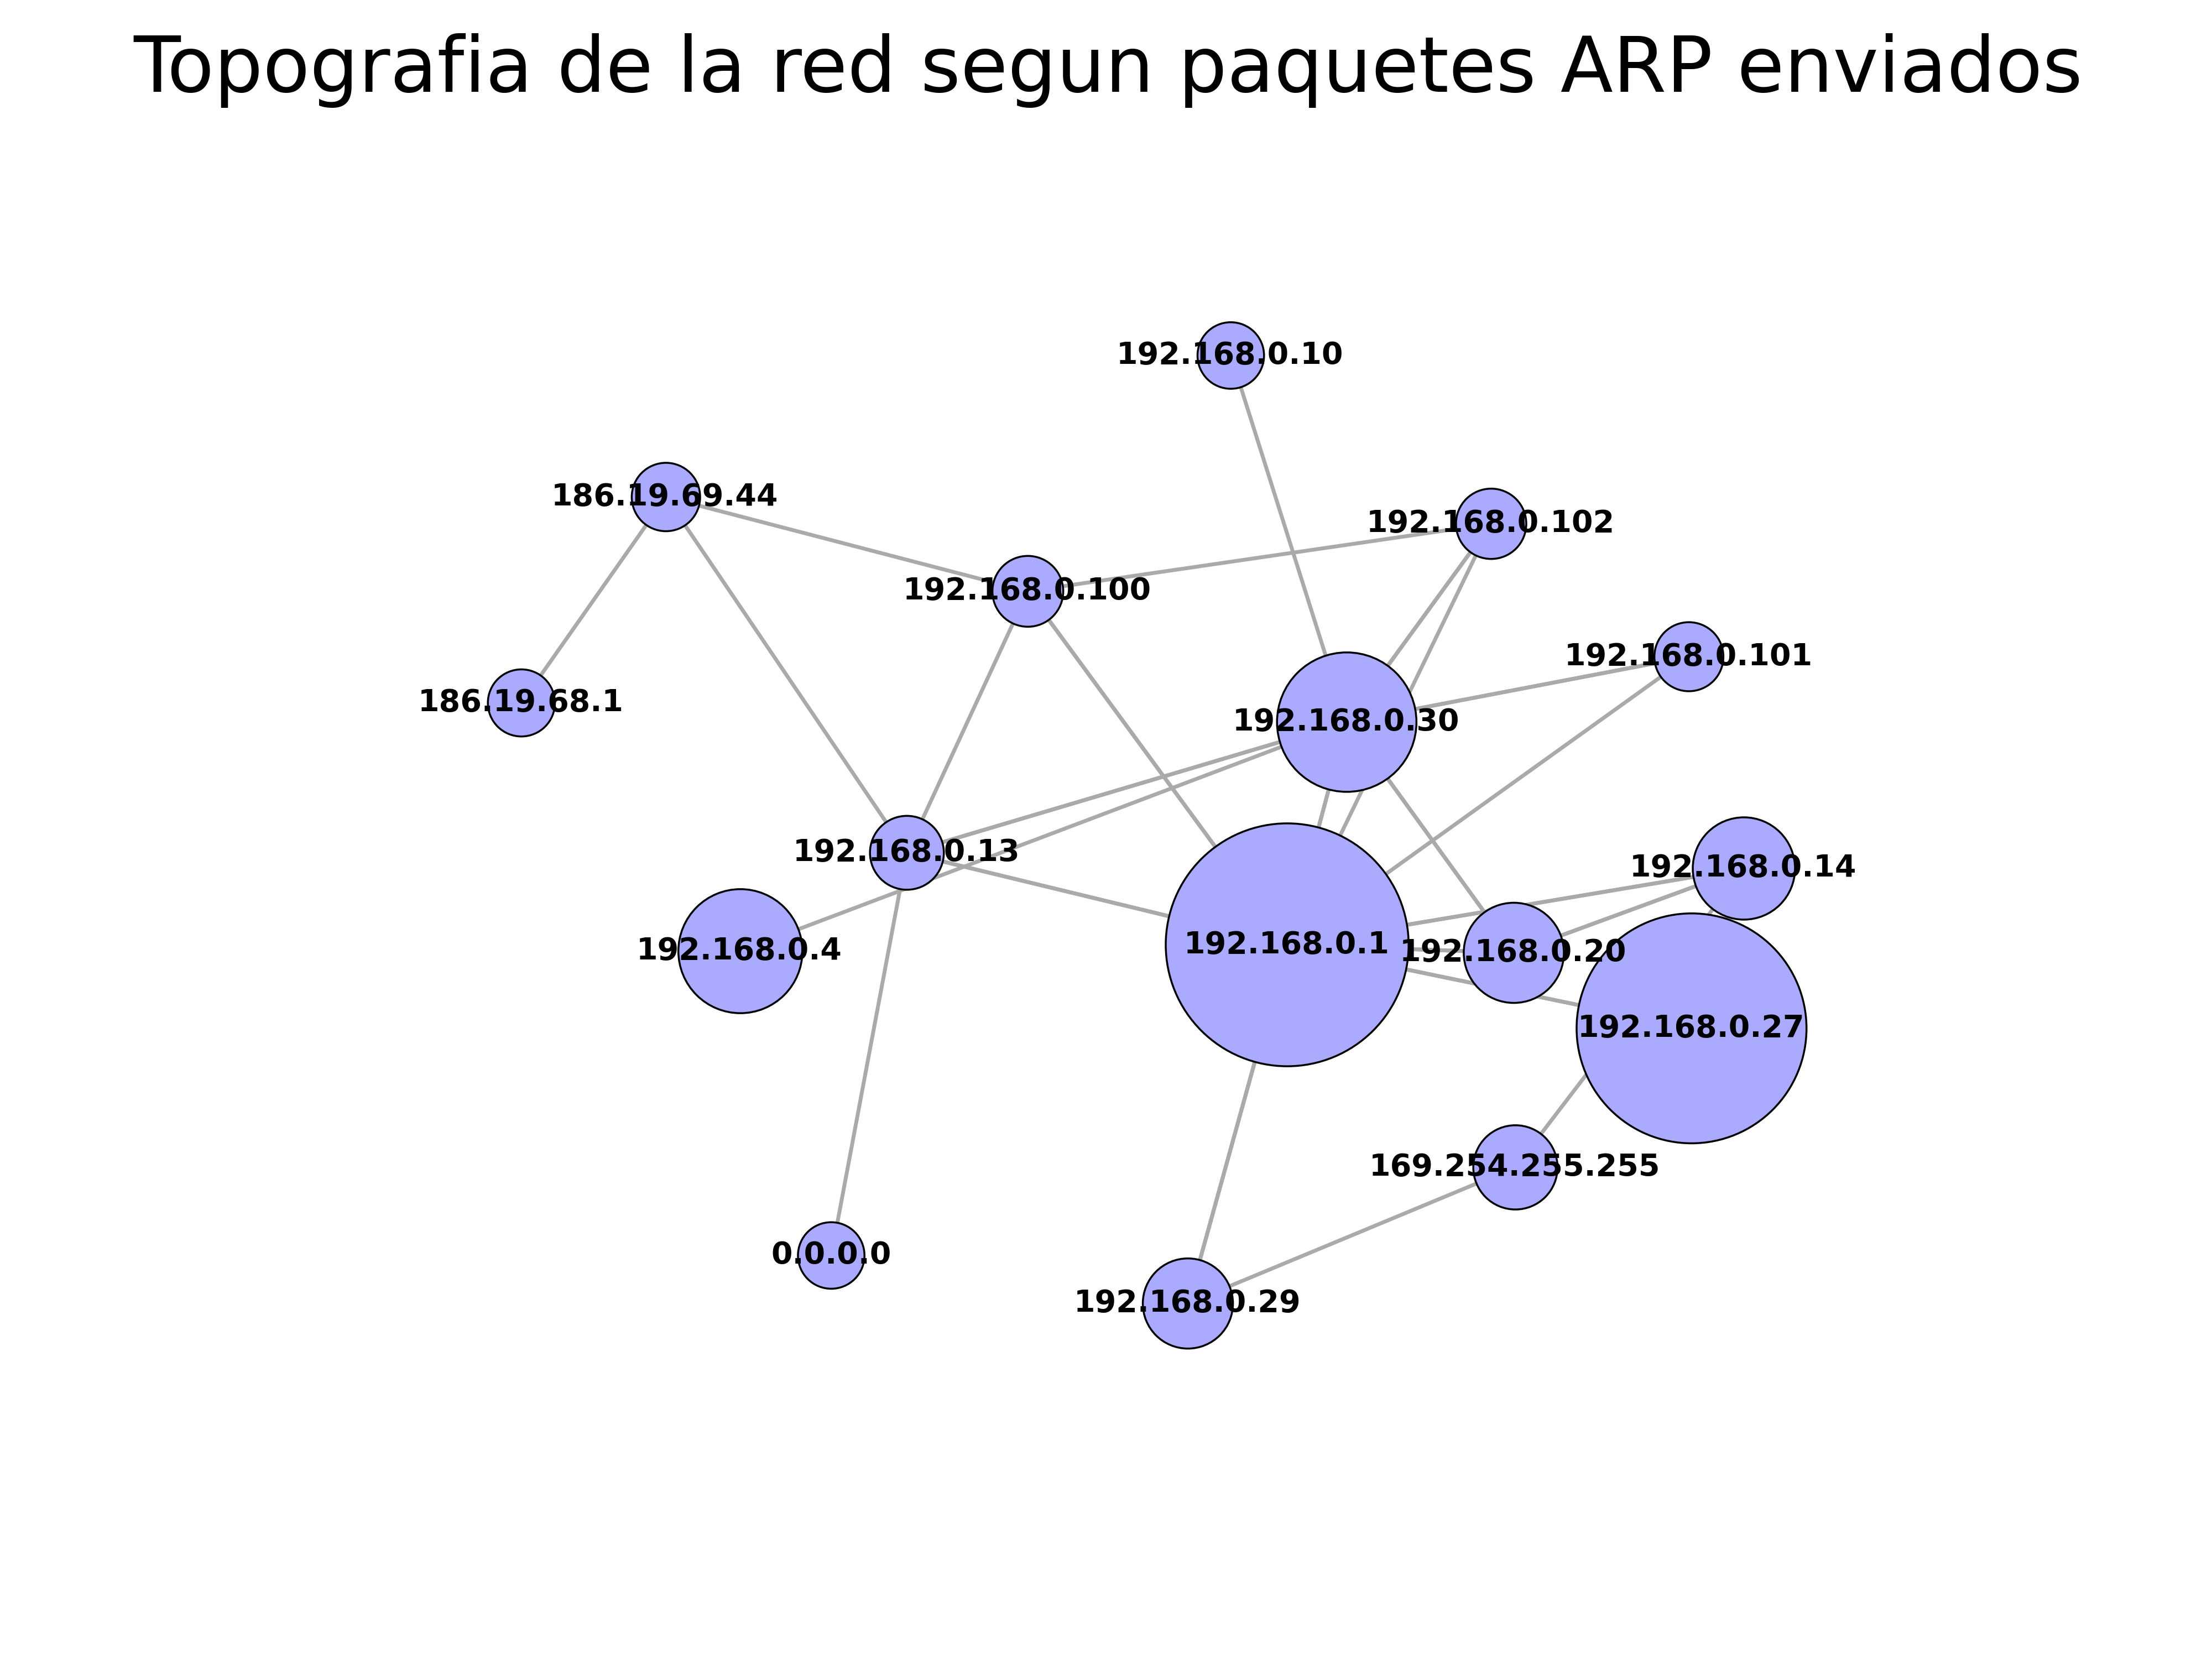
\includegraphics[width=0.7\textwidth]{graficos/red_domestica_network.png}
  \caption{}
  \label{fig:red_domestica_network}
\end{figure}

\FloatBarrier

\subsubsection{Paquetes capturados e información}

Los gráficos de torta nos permiten ver la relación entre la cantidad de paquetes y la información que provee cada nodo en la red. 

\begin{figure}[h!]
  \centering
   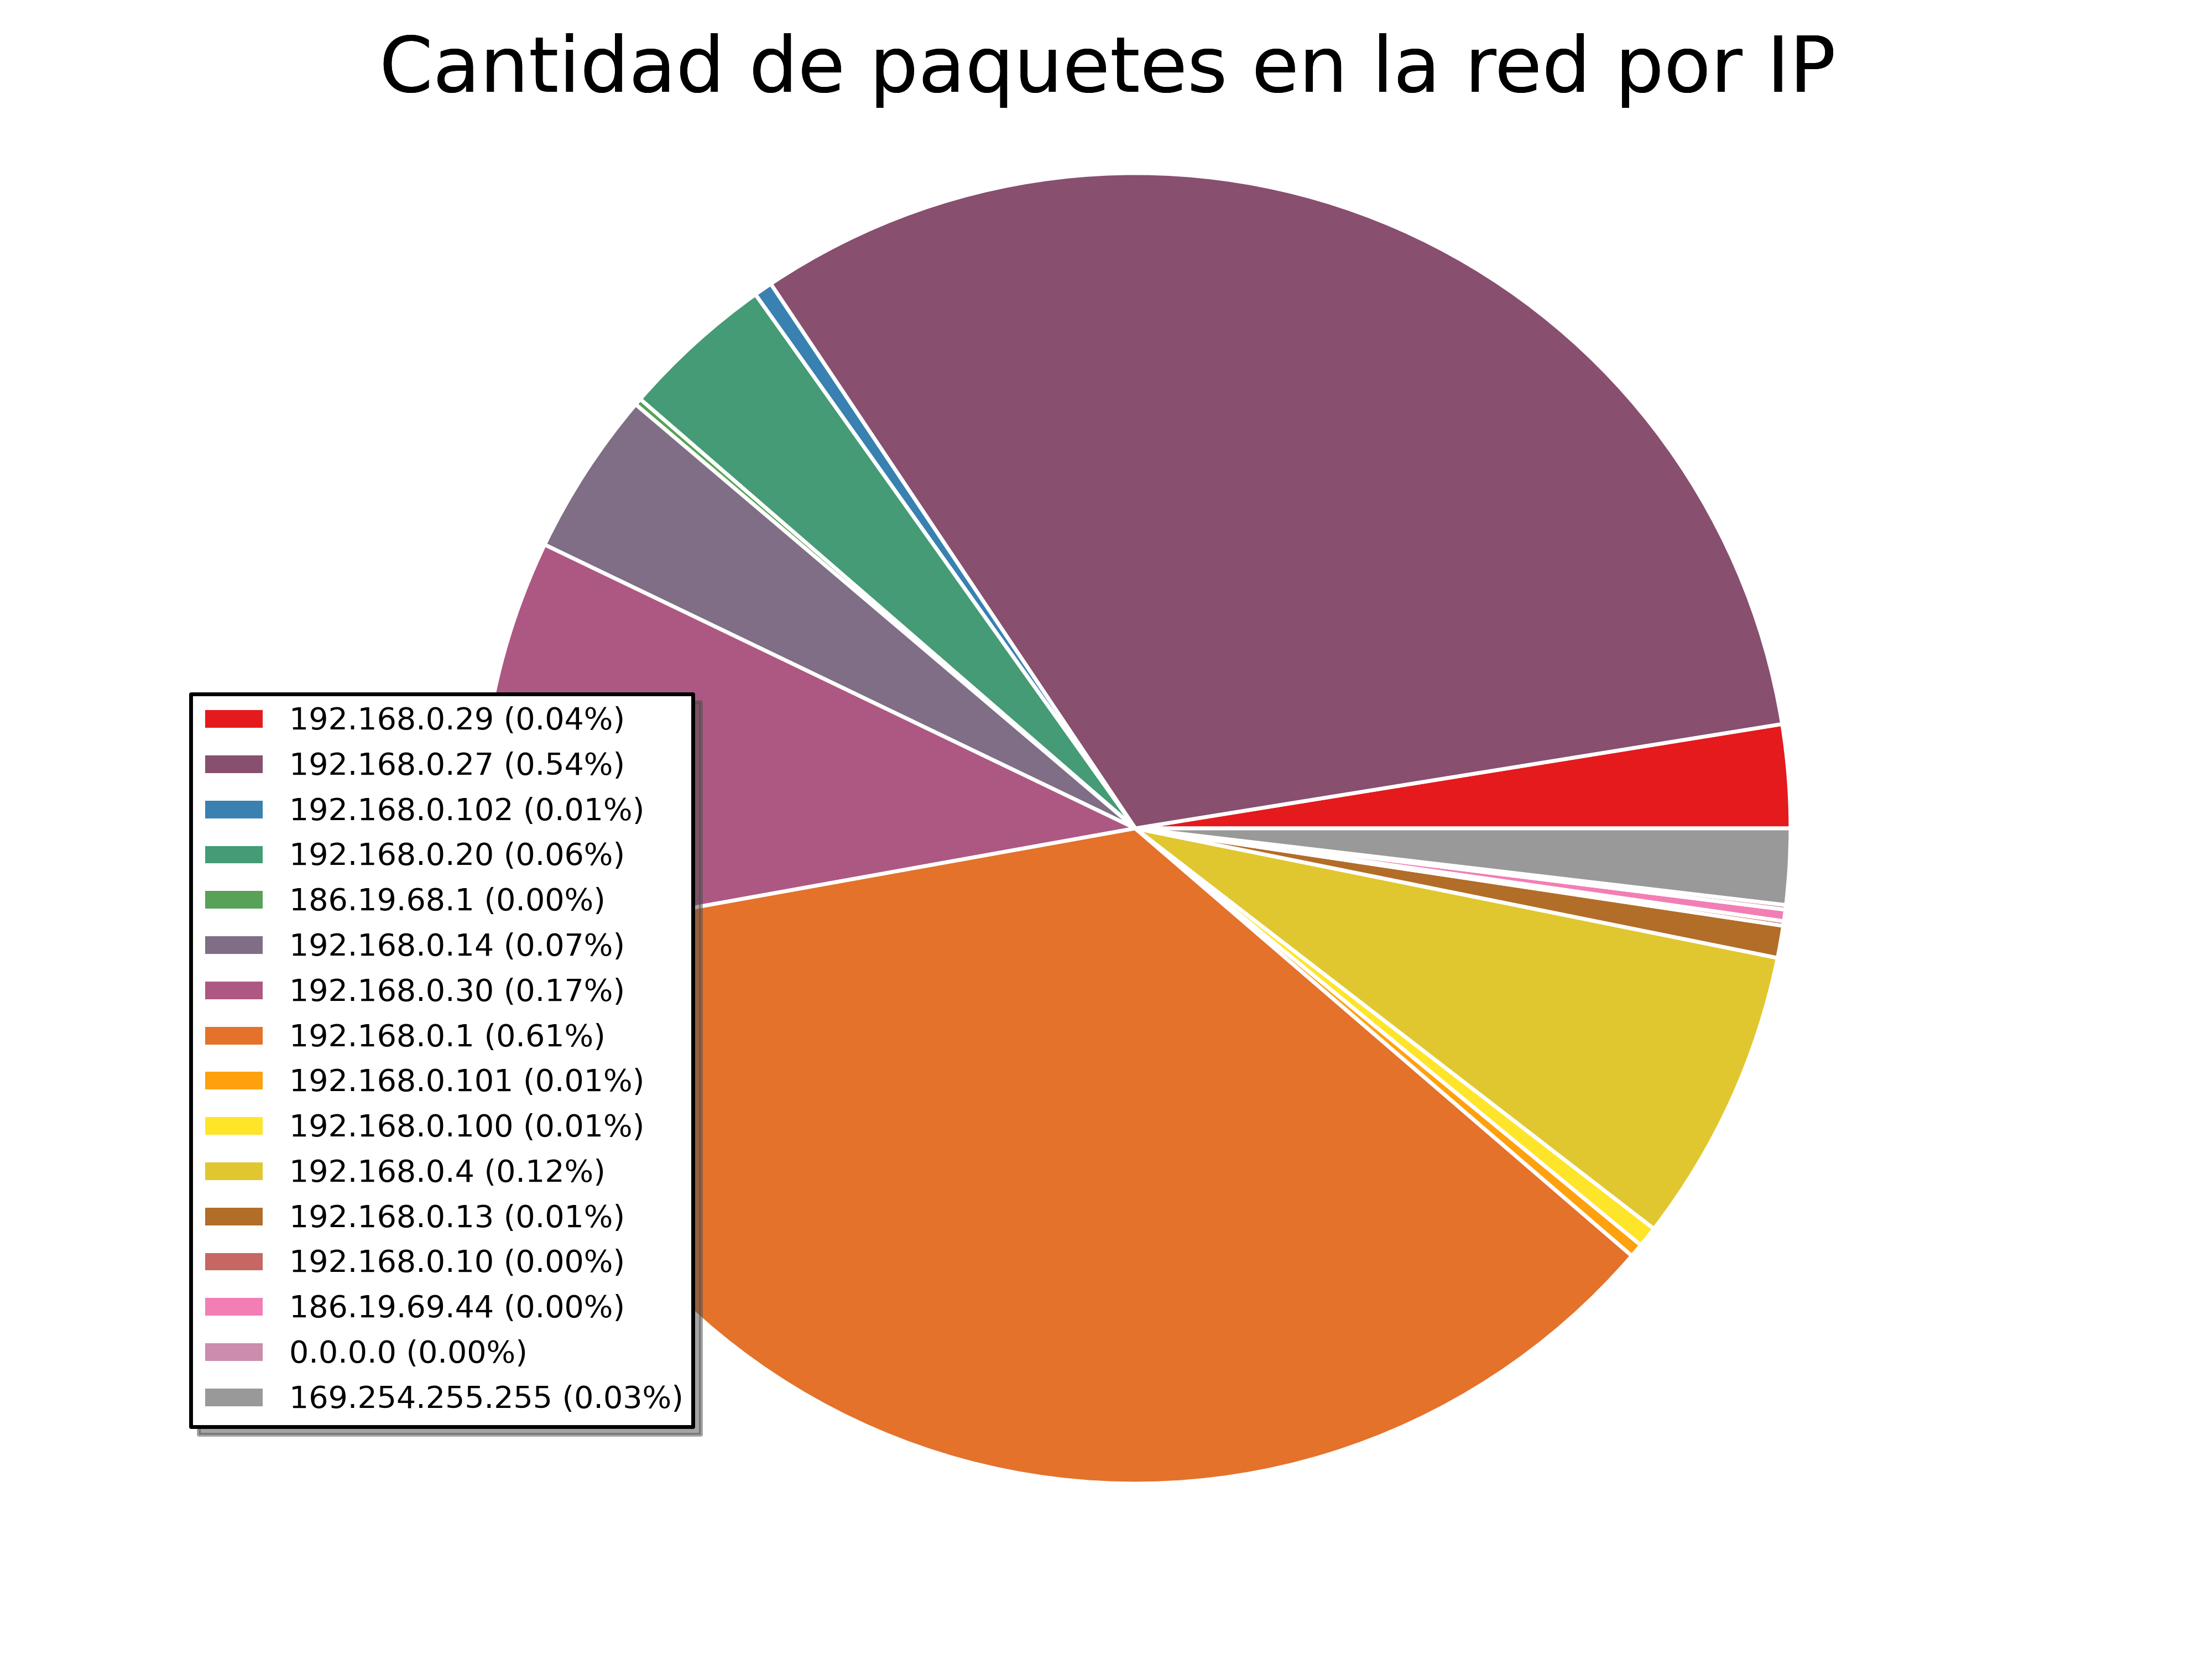
\includegraphics[width=0.7\textwidth]{graficos/red_domestica_pie_arp.png}
  \caption{}
  \label{fig:red_domestica_pie_arp}
\end{figure}

\begin{figure}[h!]
  \centering
   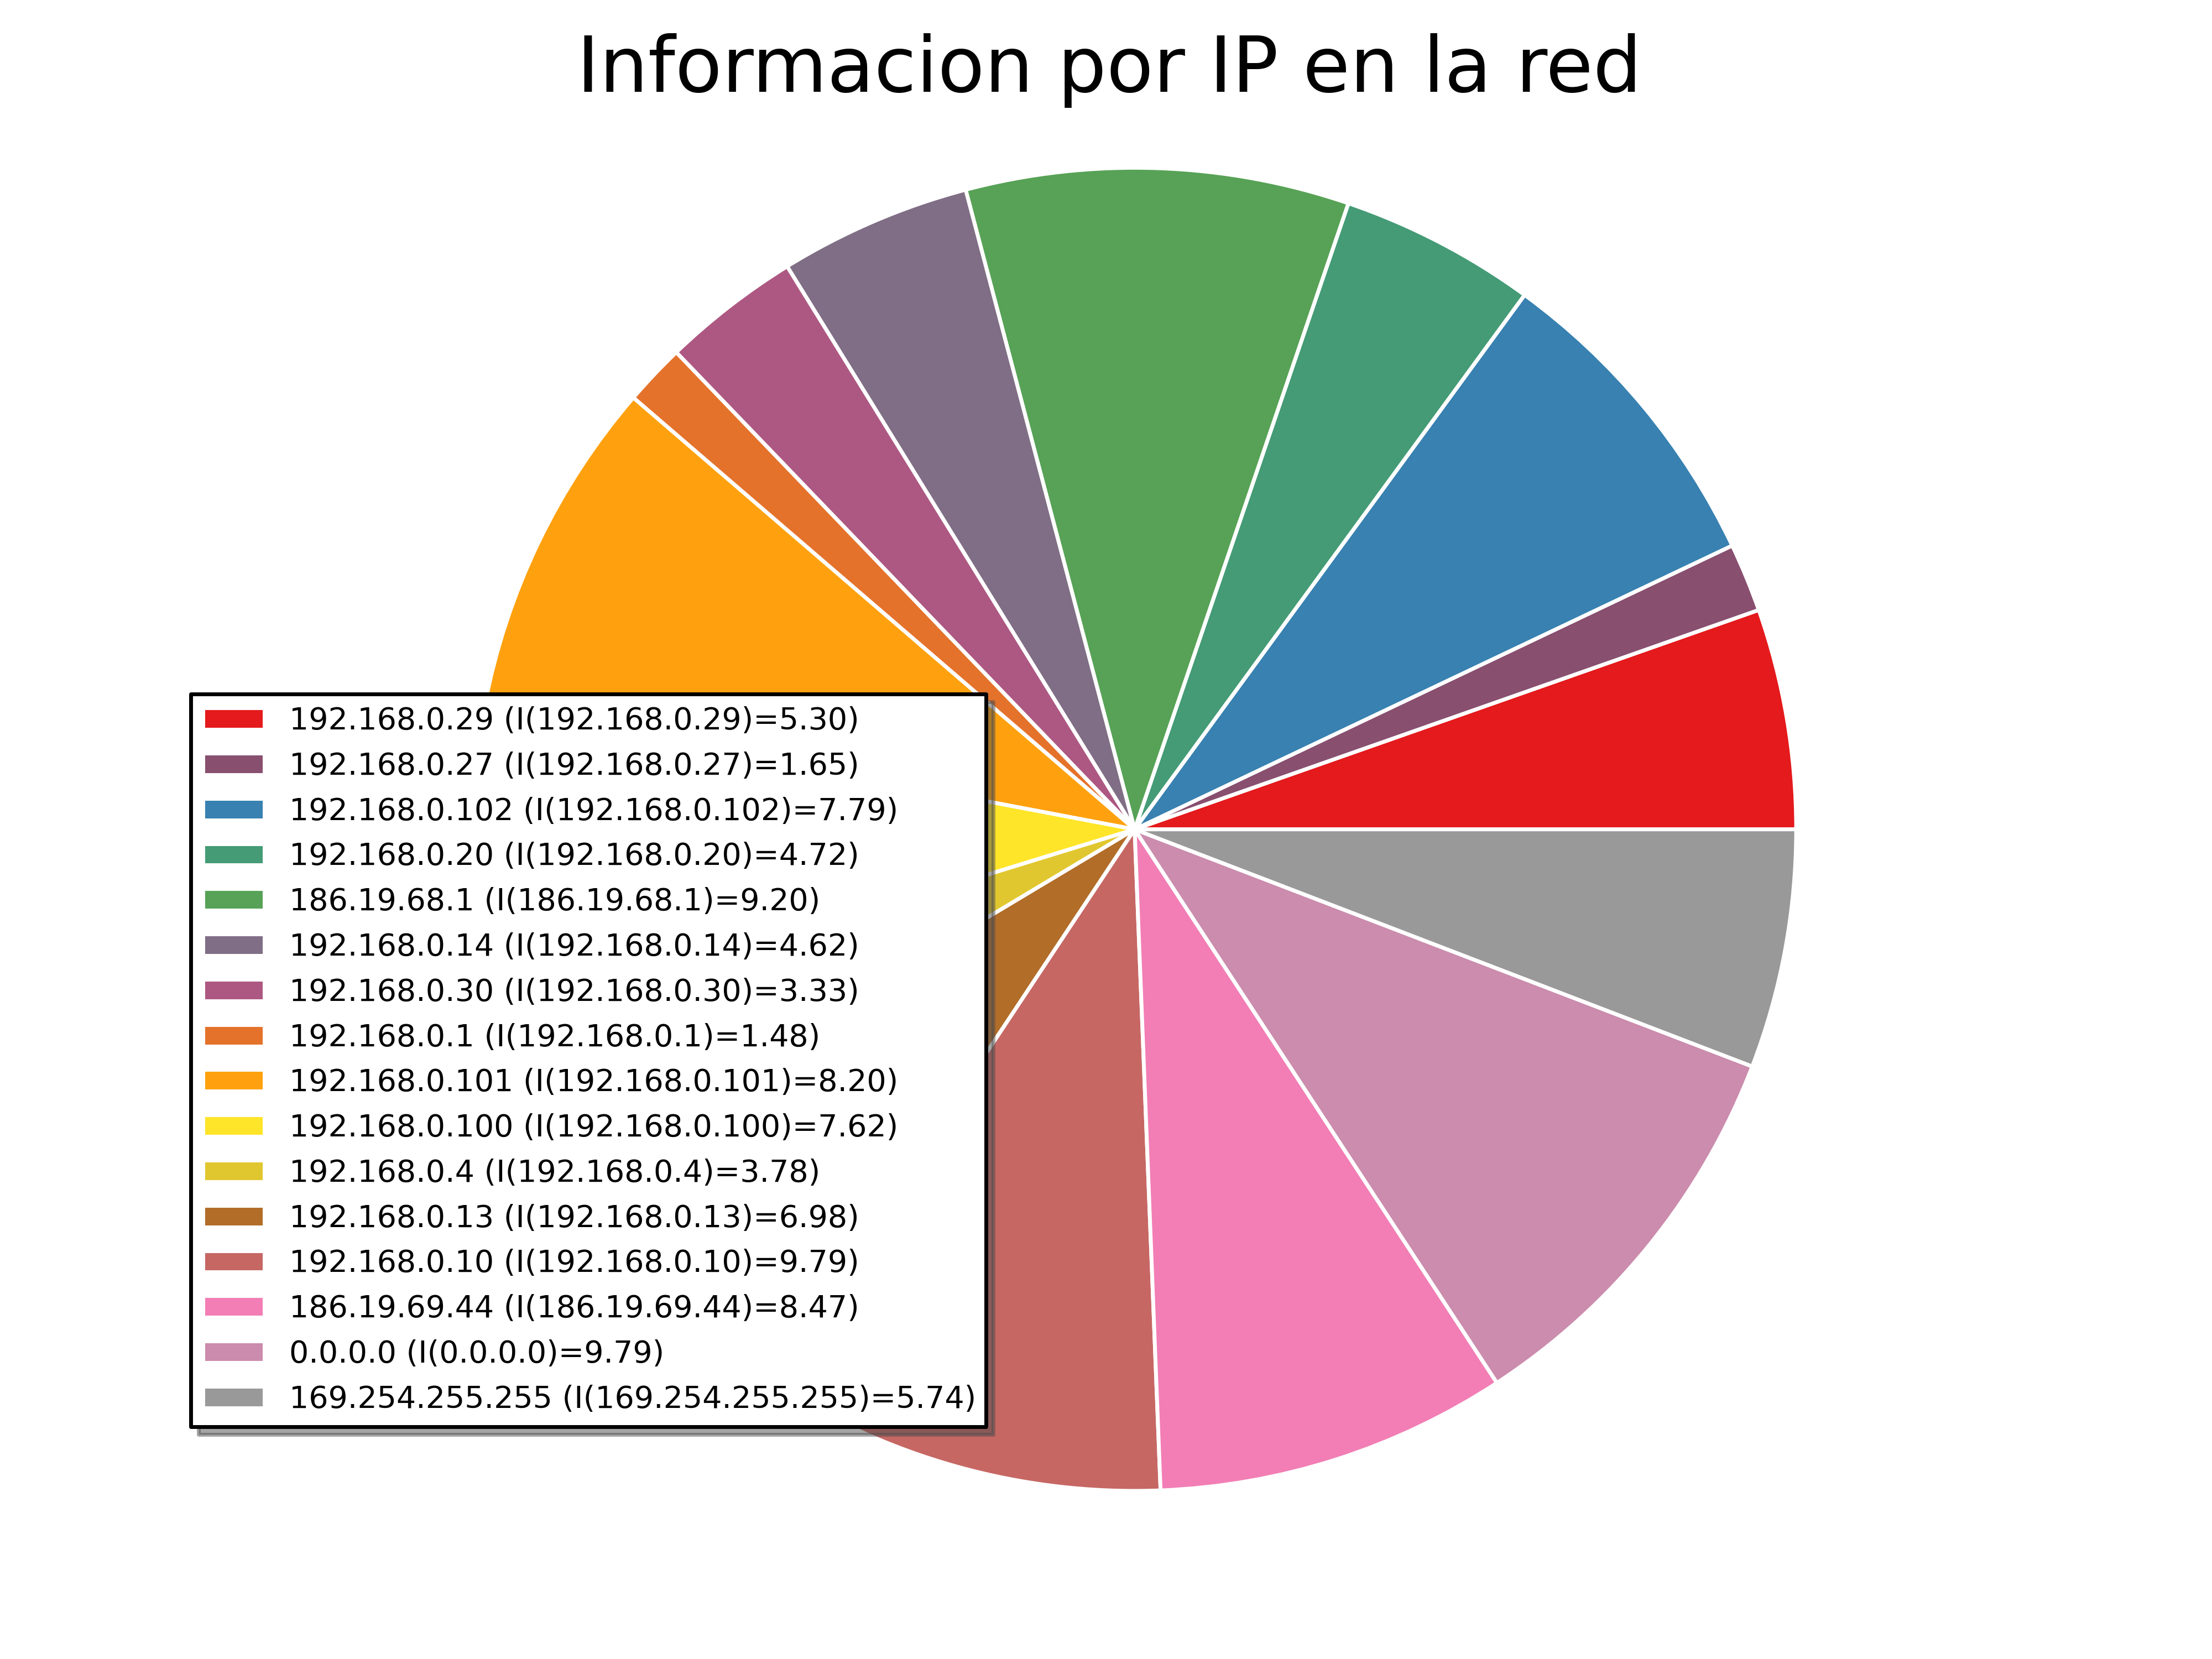
\includegraphics[width=0.7\textwidth]{graficos/red_domestica_pie_arp_information.png}
  \caption{}
  \label{fig:red_domestica_pie_arp_information}
\end{figure}

En los gráficos ~\ref{fig:red_domestica_pie_arp}. y ~\ref{fig:red_domestica_pie_arp_information}. se toma como fuente a las direcciones IP de la red.
Se puede observar que los nodos distinguidos mencionados anteriormente son los mas frecuentes y por lo tanto los que menos información presentan.
\\
A continuación analizaremos la relación entre la cantidad de paquetes y la información que provee cada tipo de paquete.

\begin{figure}[h!]
  \centering
   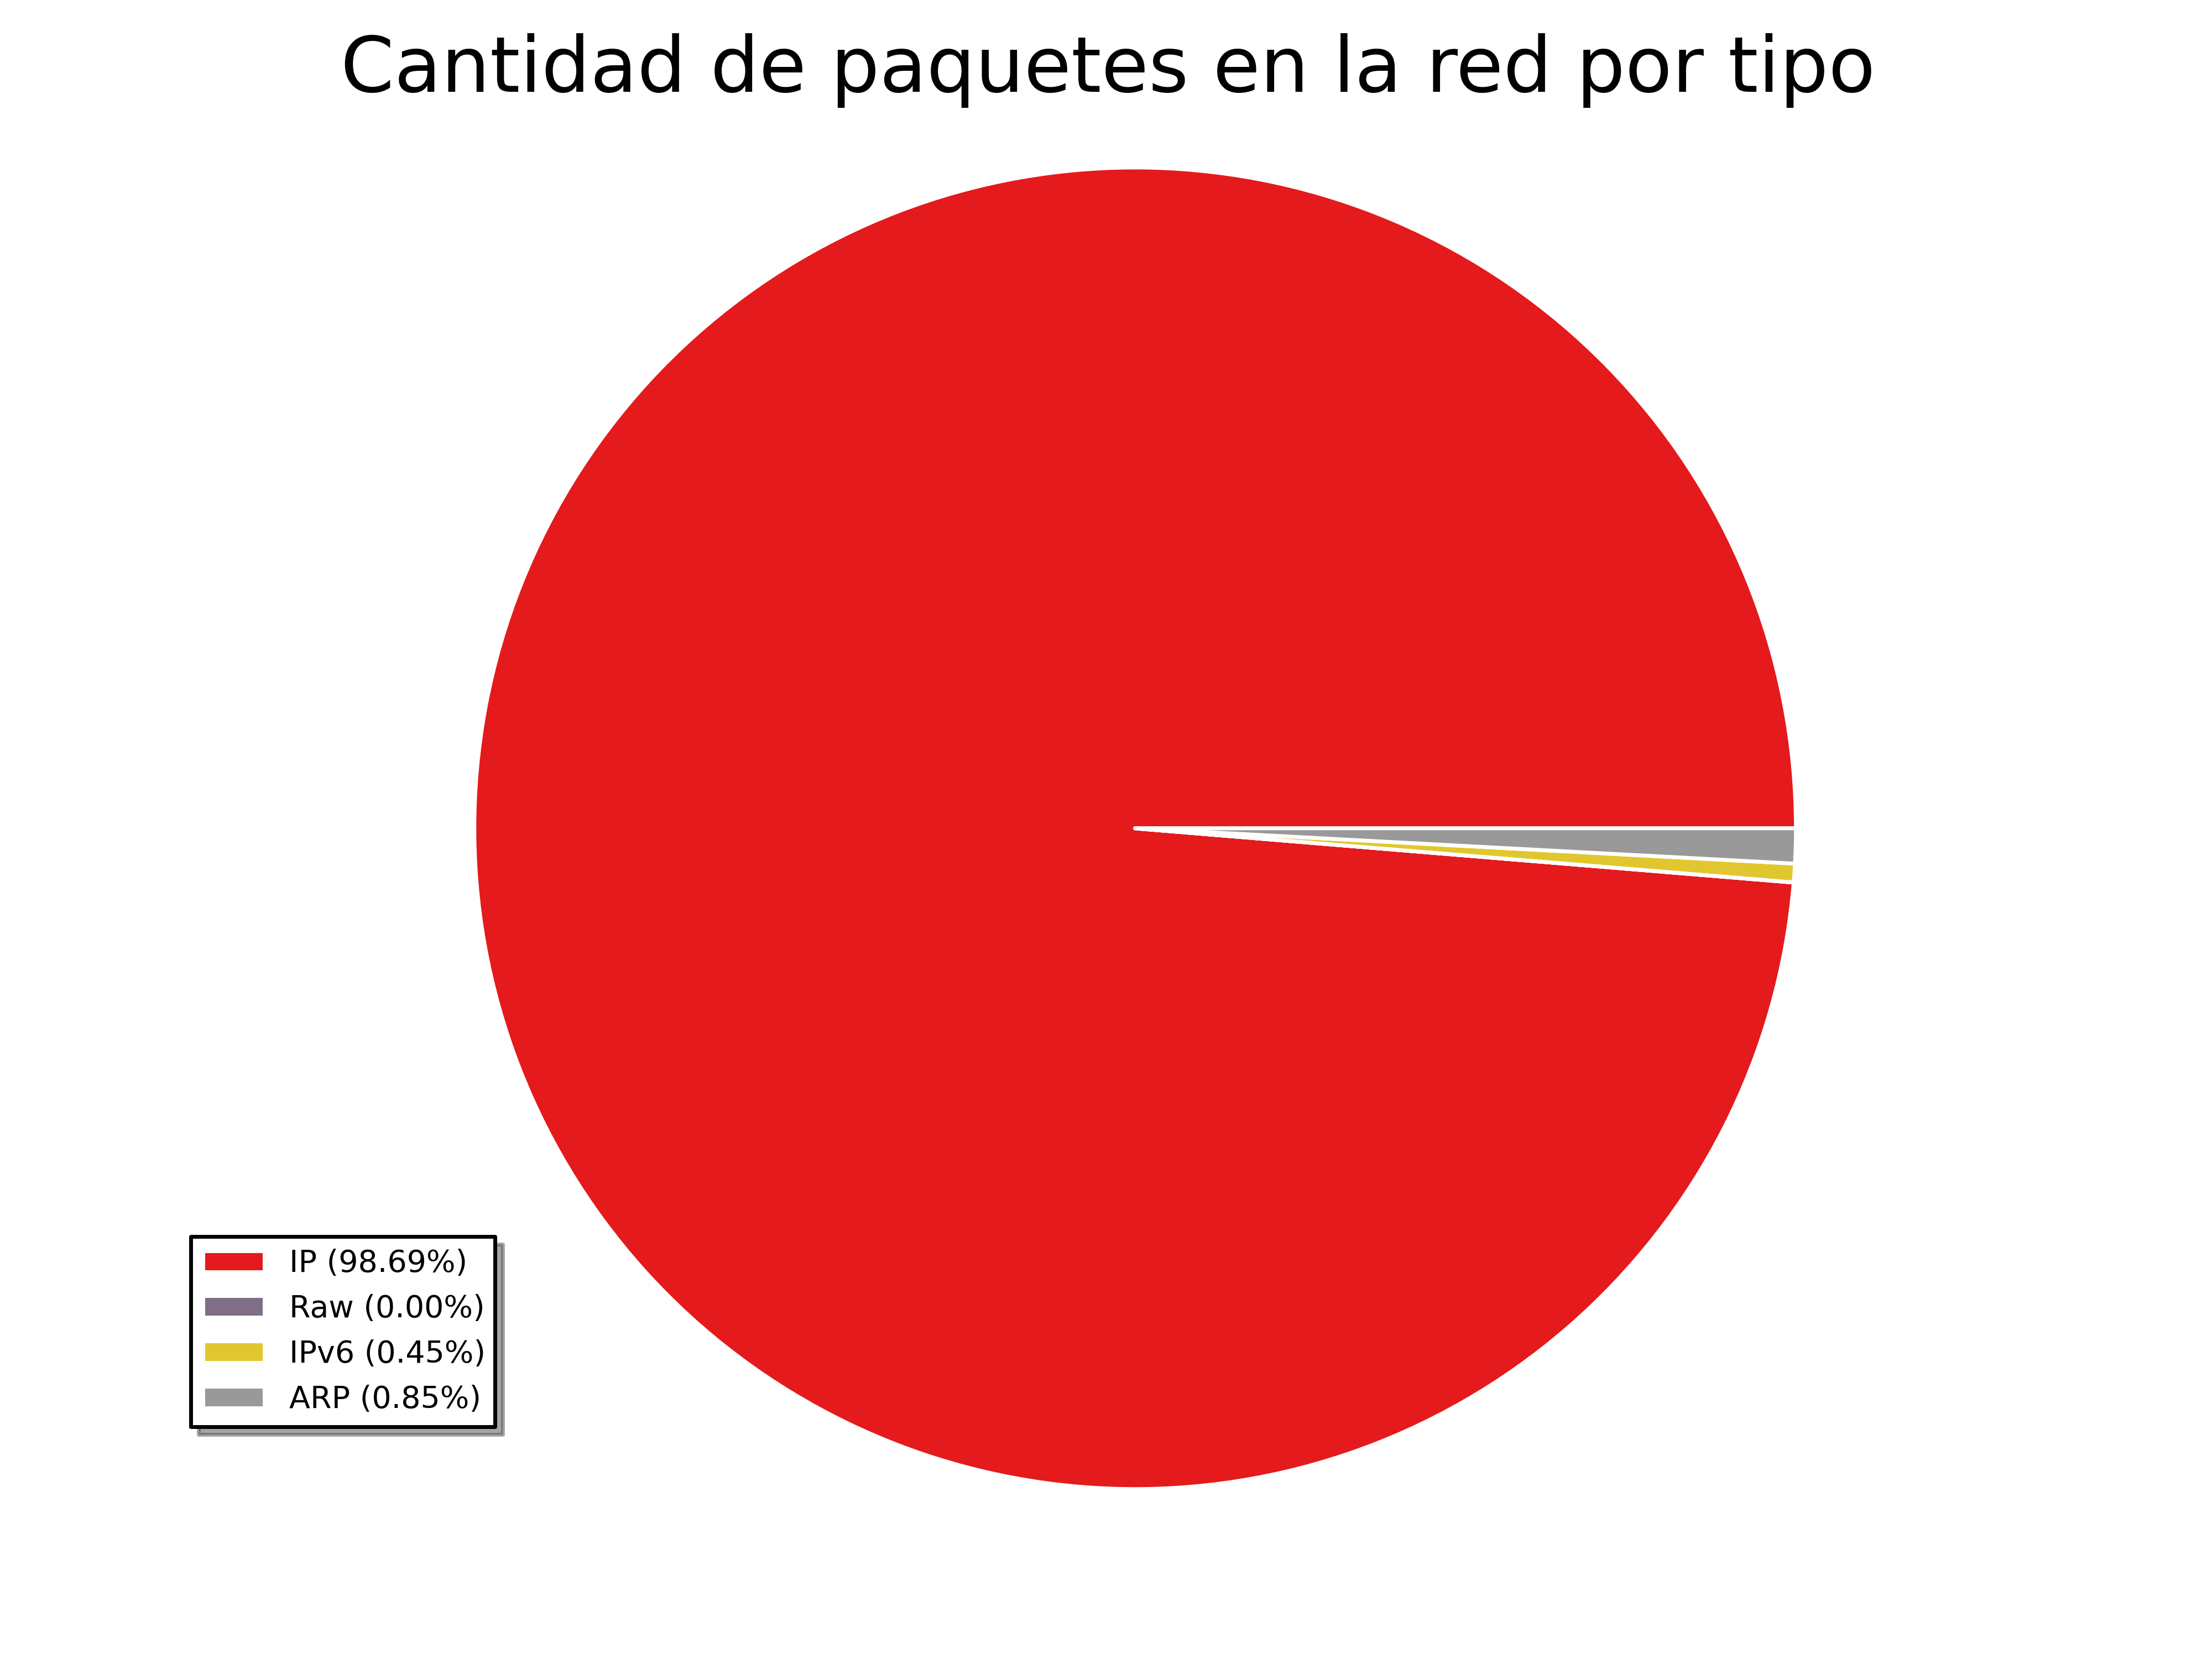
\includegraphics[width=0.7\textwidth]{graficos/red_domestica_pie_type.png}
  \caption{}
  \label{fig:red_domestica_pie_type}
\end{figure}

\begin{figure}[h!]
  \centering
   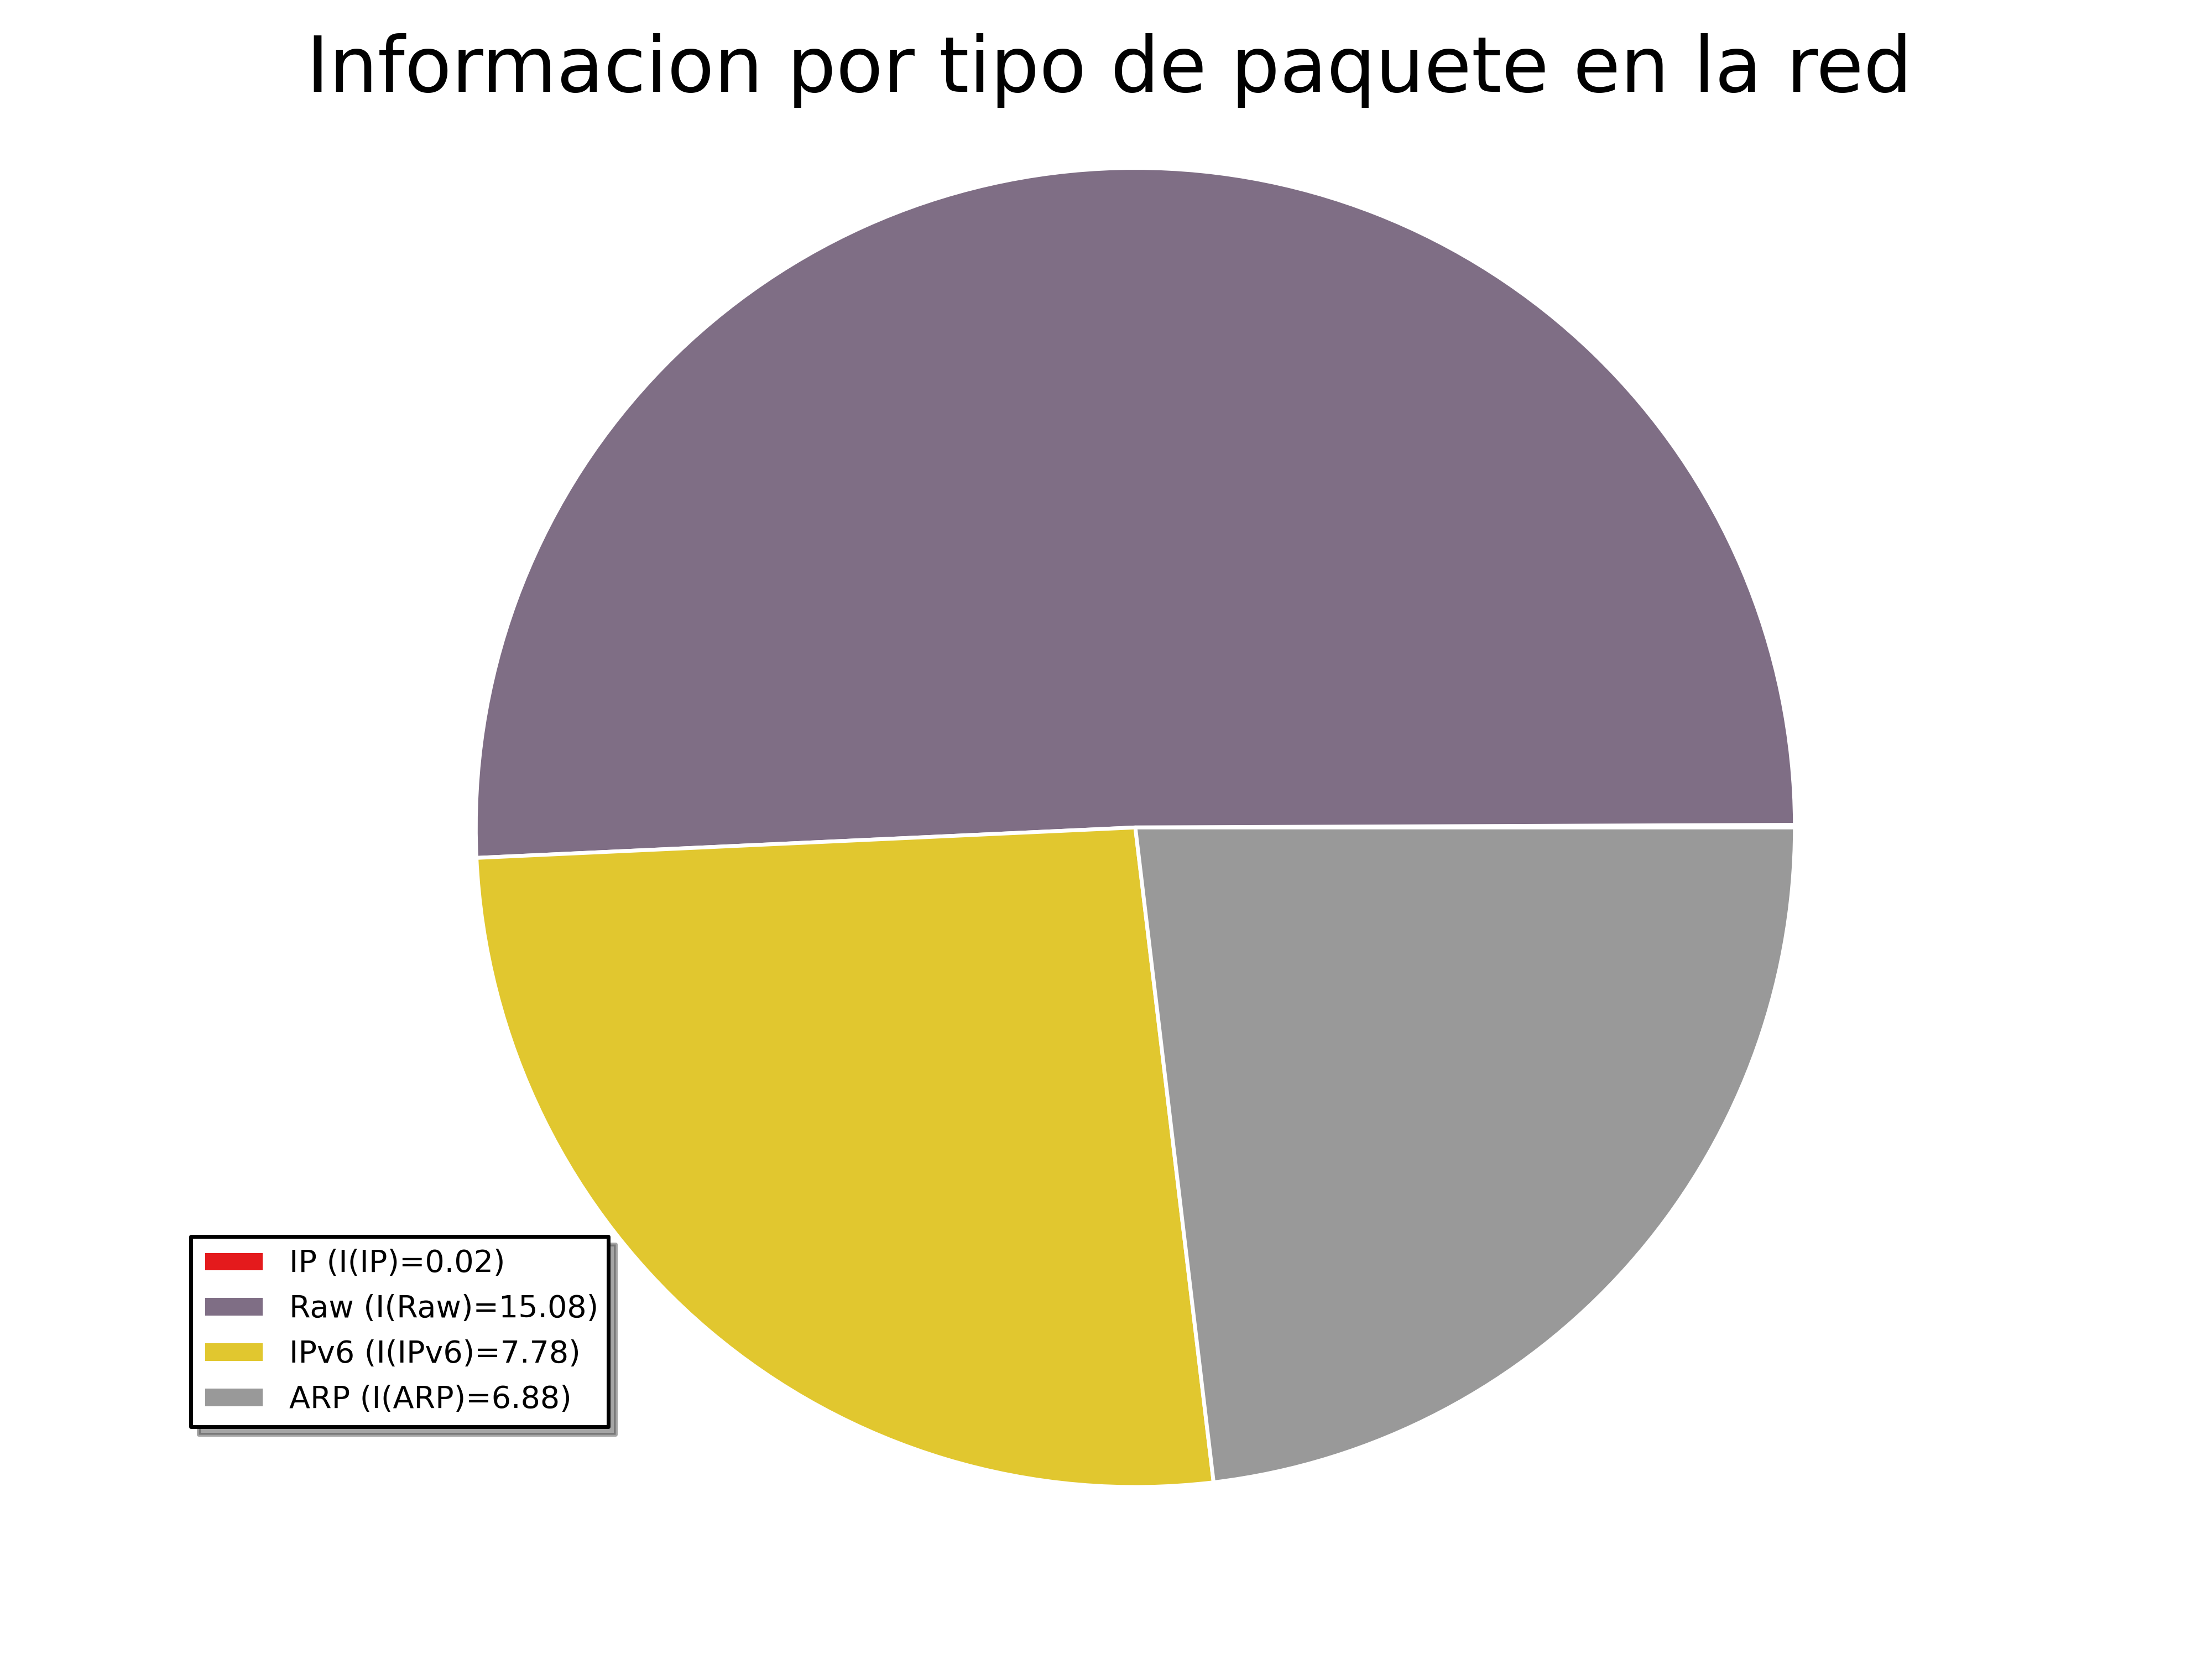
\includegraphics[width=0.7\textwidth]{graficos/red_domestica_pie_type_information.png}
  \caption{}
  \label{fig:red_domestica_pie_type_information}
\end{figure}

En los gráficos ~\ref{fig:red_domestica_pie_type}. y ~\ref{fig:red_domestica_pie_type_information}. la fuente es la indicada en la cátedra. 
Se observa que el protocolo que que presenta mayor frecuencia es el IP con un porcentaje muy superior al resto y que por el contrario, aporta muy poca información. En este caso el símbolo distinguido en esta fuente sería el que representa al tipo de paquete IP.

\subsubsection{Histogramas (de IPs y protocolos)}

A continuación analizaremos histogramas con cortes en los valores de entropia, tanto para las IP de la red como para los tipos de protocolo.

\begin{figure}[h!]
  \centering
   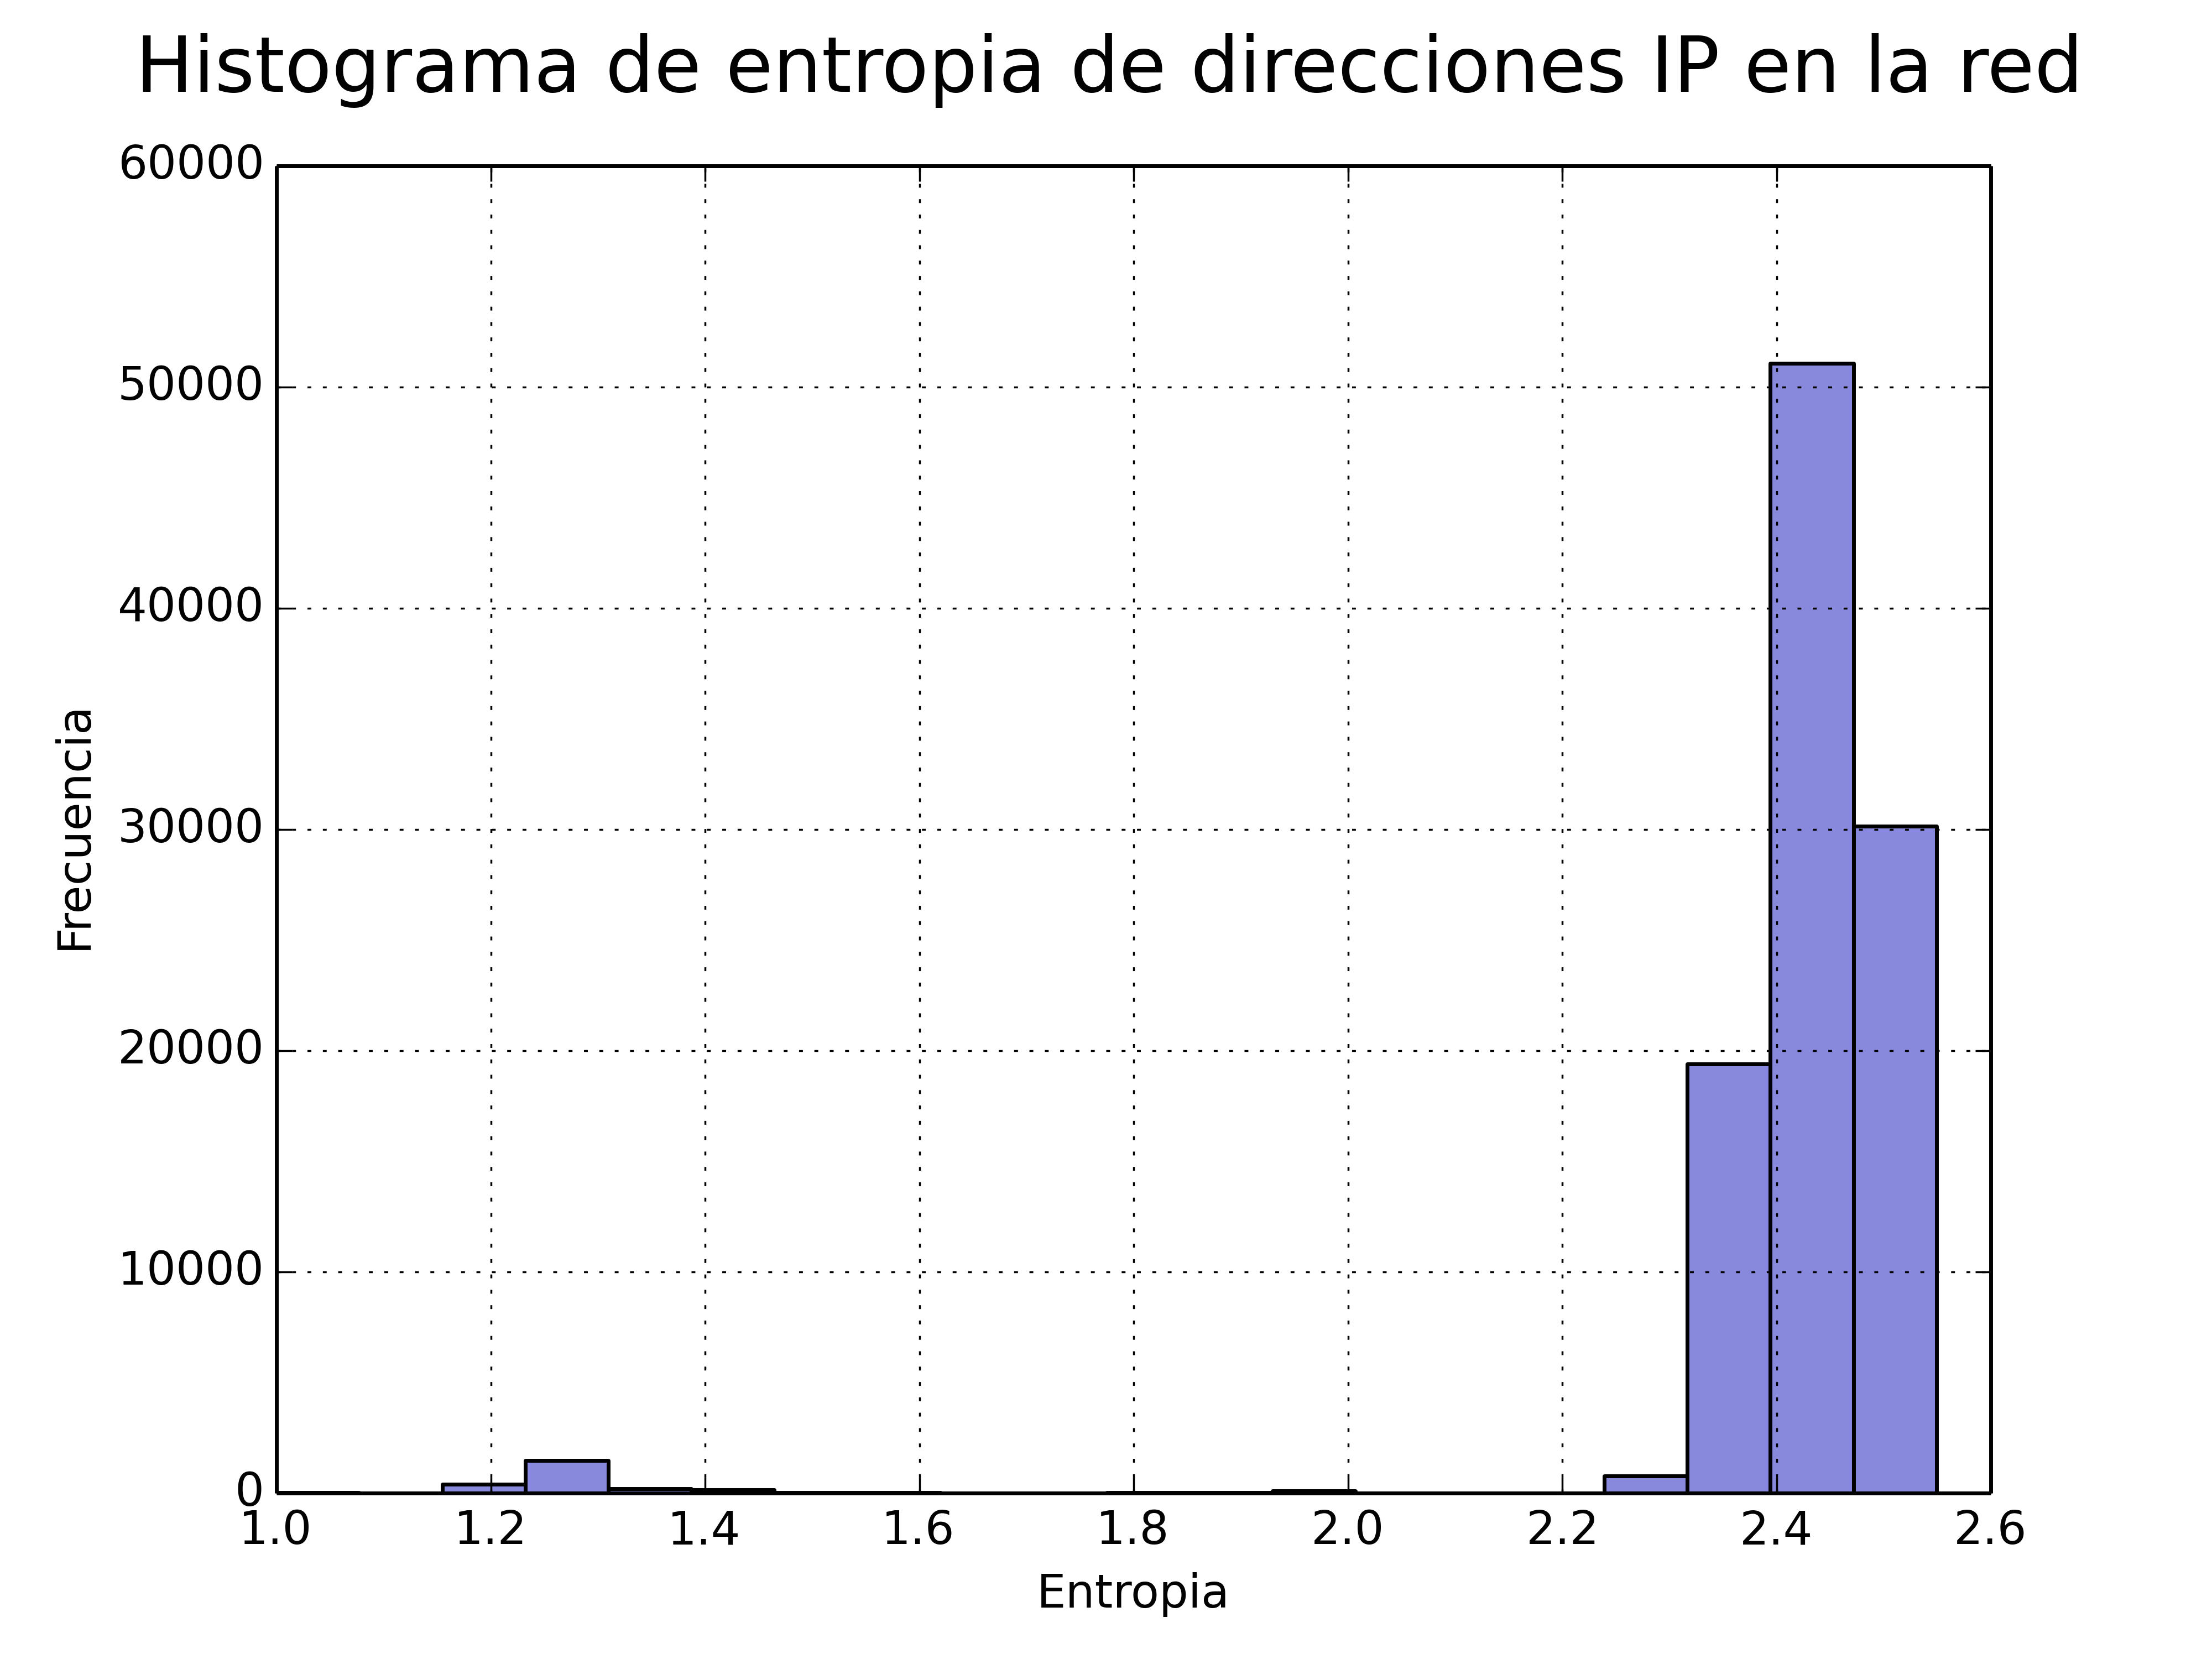
\includegraphics[width=0.7\textwidth]{graficos/red_domestica_hist_arp.png}
  \caption{Mi Figura}
  \label{fig:red_domestica_hist_arp}
\end{figure}

\begin{figure}[h!]
  \centering
   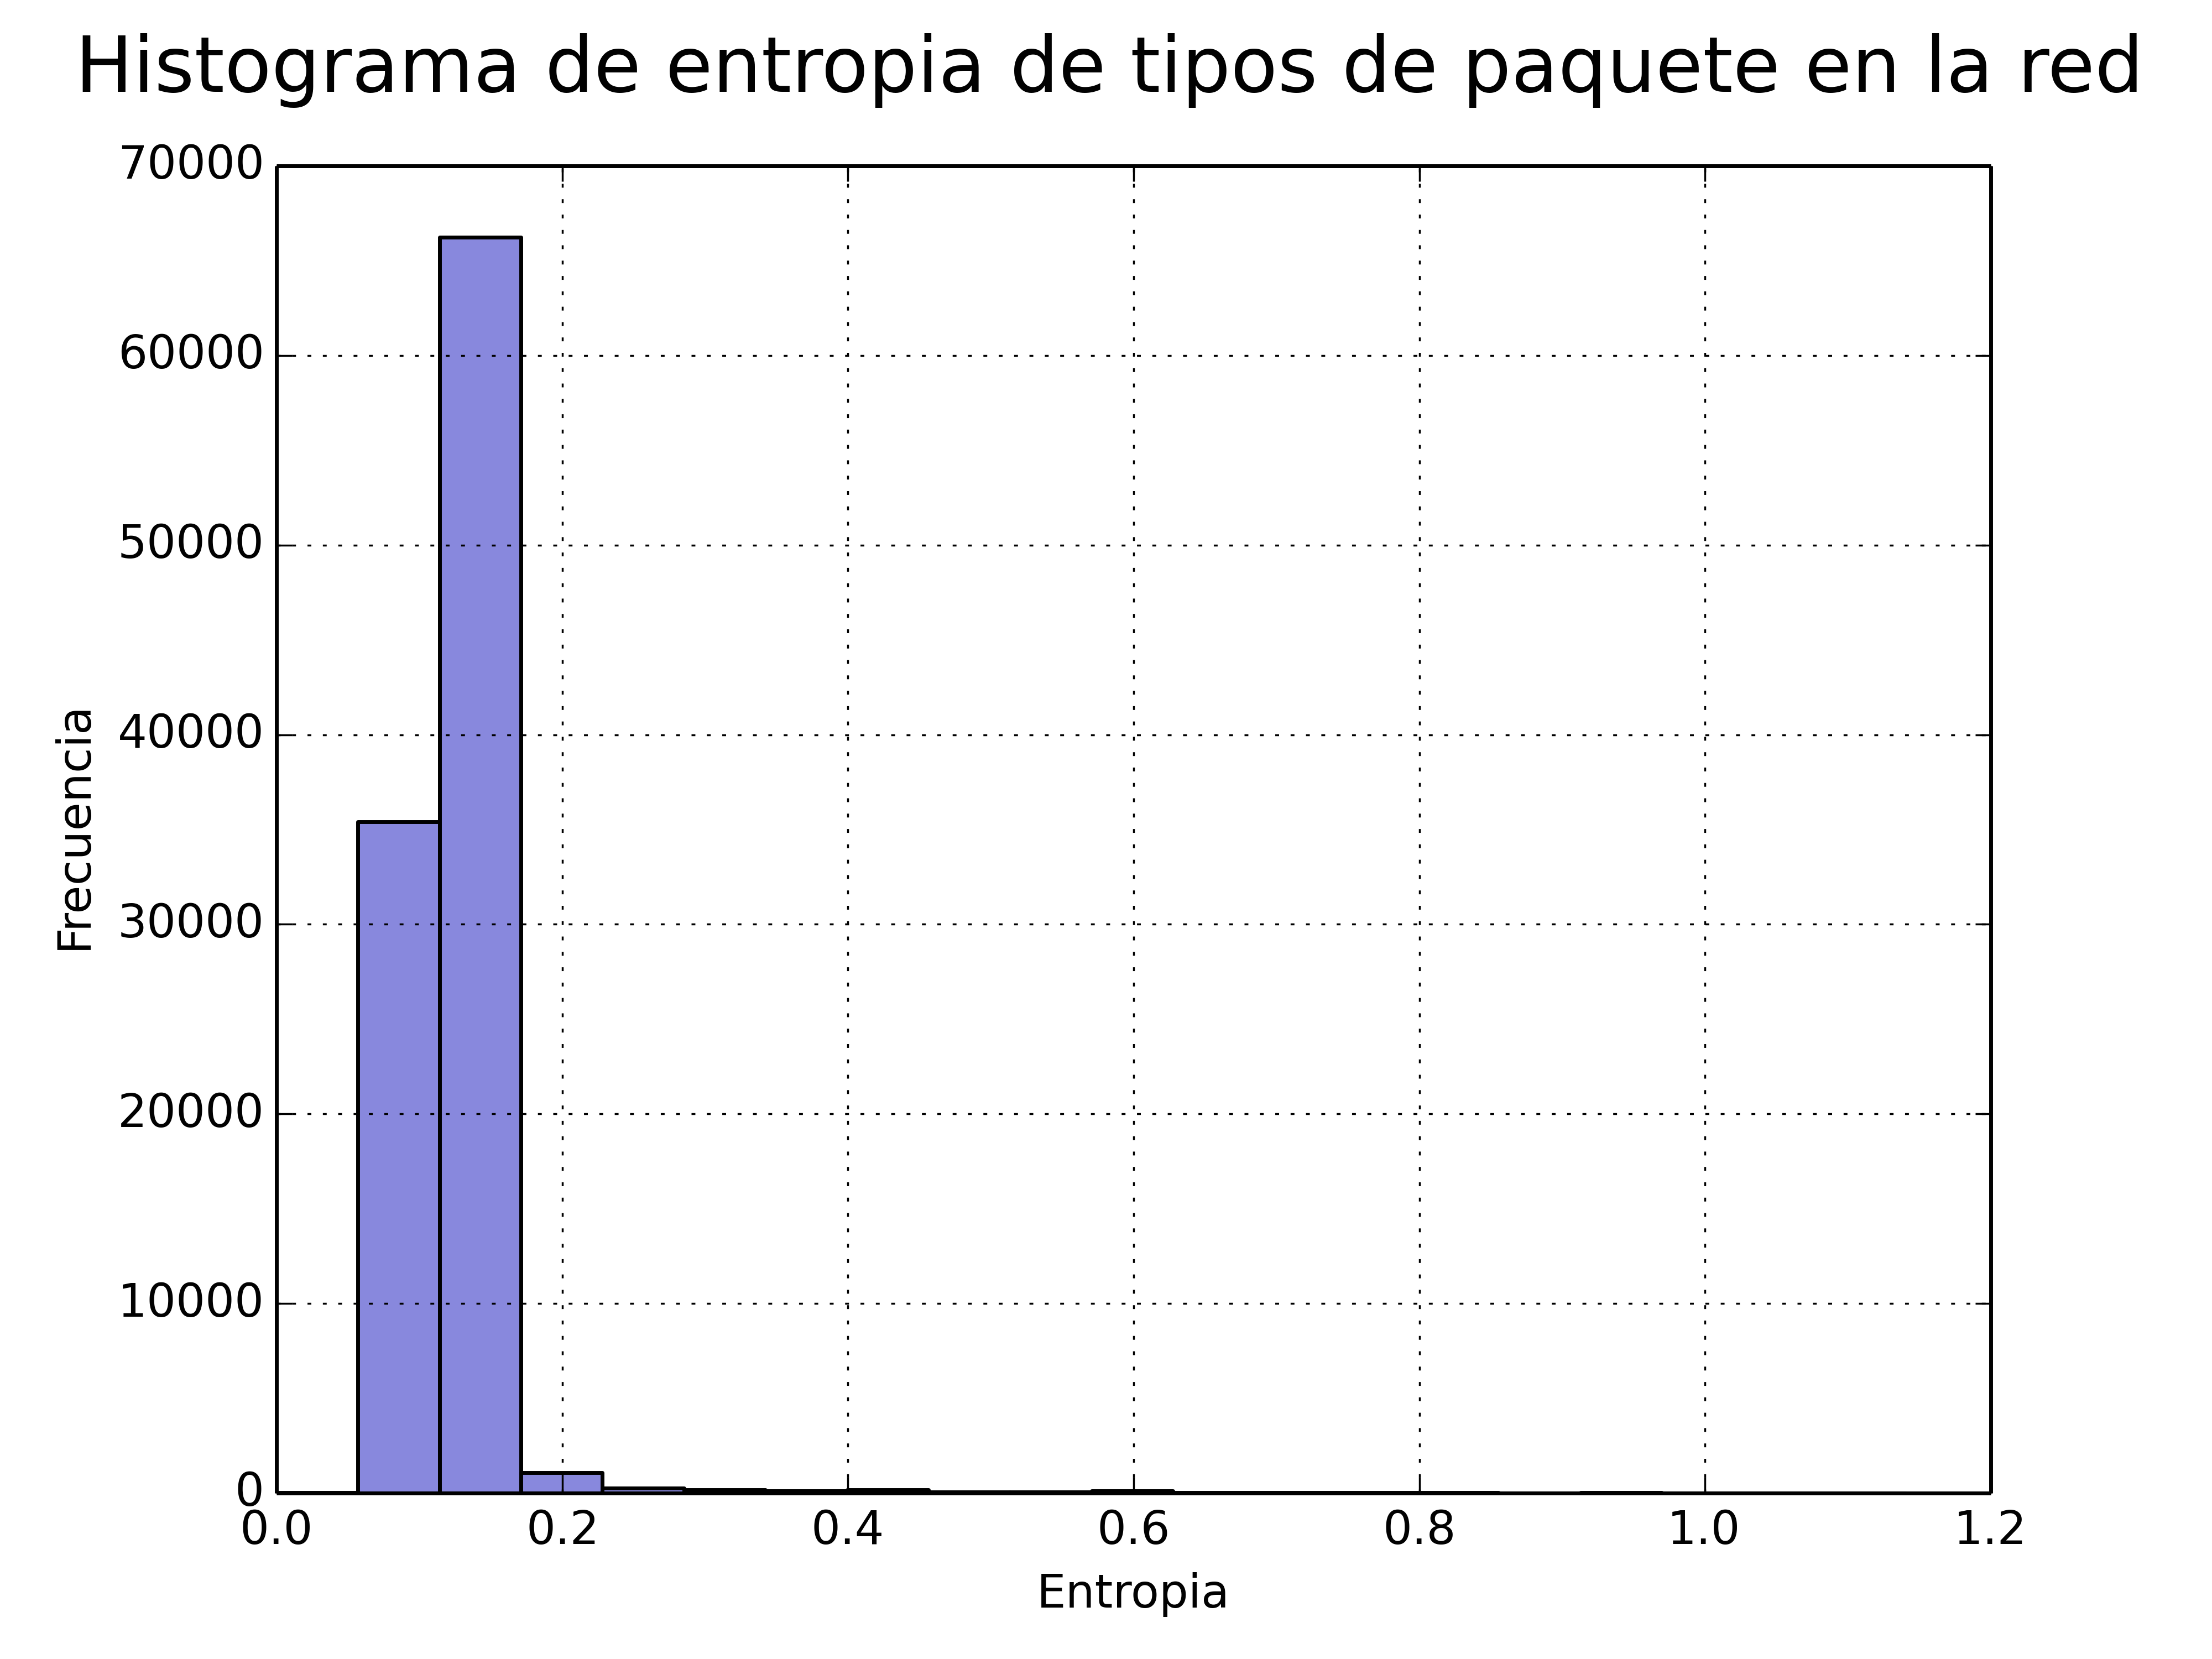
\includegraphics[width=0.7\textwidth]{graficos/red_domestica_hist_type.png}
  \caption{Mi Figura}
  \label{fig:red_domestica_hist_type}
\end{figure}

Podemos observar que para el caso de la captura de paquetes de la fuente de IPs se presenta una entropía media mayor que en la fuente por tipo protocolo. Esto se debe a la impredecibilidad de los símbolos en el caso de las IP en comparación con la de los protocolos, donde la mayoría de los paquetes eran de tipo IP.

